%----------------------------------------------------------------------------------------
%	Inställningar och dokumentkonfiguration
%----------------------------------------------------------------------------------------

\documentclass[paper=a4, fontsize=11pt]{report} % A4-sida och 11 punkters fontstorlek

\usepackage[T1]{fontenc} % 8-bitarskodning som har 256 glyfer
\usepackage[swedish]{babel} % Svenskt språk
\usepackage[utf8]{inputenc} % För svenska tecken
\usepackage{dtklogos} % Logos
\usepackage{wallpaper} % Bakgrundsbild
\usepackage{fancyhdr} % Specialsidhuvud och sidfot
\usepackage{enumerate} 
\usepackage{xifthen}% provides \isempty test
\usepackage{listings}% Code examples
\usepackage{xcolor}
\newcounter{tmpc}
\lstdefinestyle{BashInputStyle}{
  language=bash,
  basicstyle=\footnotesize\ttfamily,
  numbers=left,
  numberstyle=\tiny,
  numbersep=3pt,
  frame=tb,
  columns=fullflexible,
  backgroundcolor=\color{yellow!20},
  linewidth=0.9\linewidth,
  xleftmargin=0.1\linewidth
}
% Exampels
% Inline
% \lstinline[style=BashInputStyle]´# apt-get --purge remove rubygems´.
% Multiline
% \begin{lstlisting}[style=BashInputStyle]
%    # apt-get --purge remove rubygems
% \end{lstlisting}

\pagestyle{fancyplain} % Använd sidhuvud och sidfot på alla sidor
\fancyhead[L]{Seminar 2 -- 1DV720 -- \the\year -- Server Administration} % Titel till vänster i sidhuvud
\fancyhead[C]{} % Tomt i mitten
\fancyhead[R]{} % Tomt till höger
\fancyfoot[L]{} % Tomt till vänster
\fancyfoot[C]{} % Tomt i mitten
\fancyfoot[R]{\thepage} % Sidnumrering till höger i sidfoten
\renewcommand\thesection{\arabic{section}} % Section beter sig som i dokumentklassen article

\newcommand{\win}[1]{Microsoft Windows Server\ifthenelse{\isempty{#1}}{}{ #1}}
\newcommand{\gui}[0]{``Server with a GUI''}
\newcommand{\core}[0]{Windows Server Core}
%----------------------------------------------------------------------------------------
%	TITLE SECTION
%----------------------------------------------------------------------------------------
\newcommand\BackgroundPic{
    \put(-50,-50){
    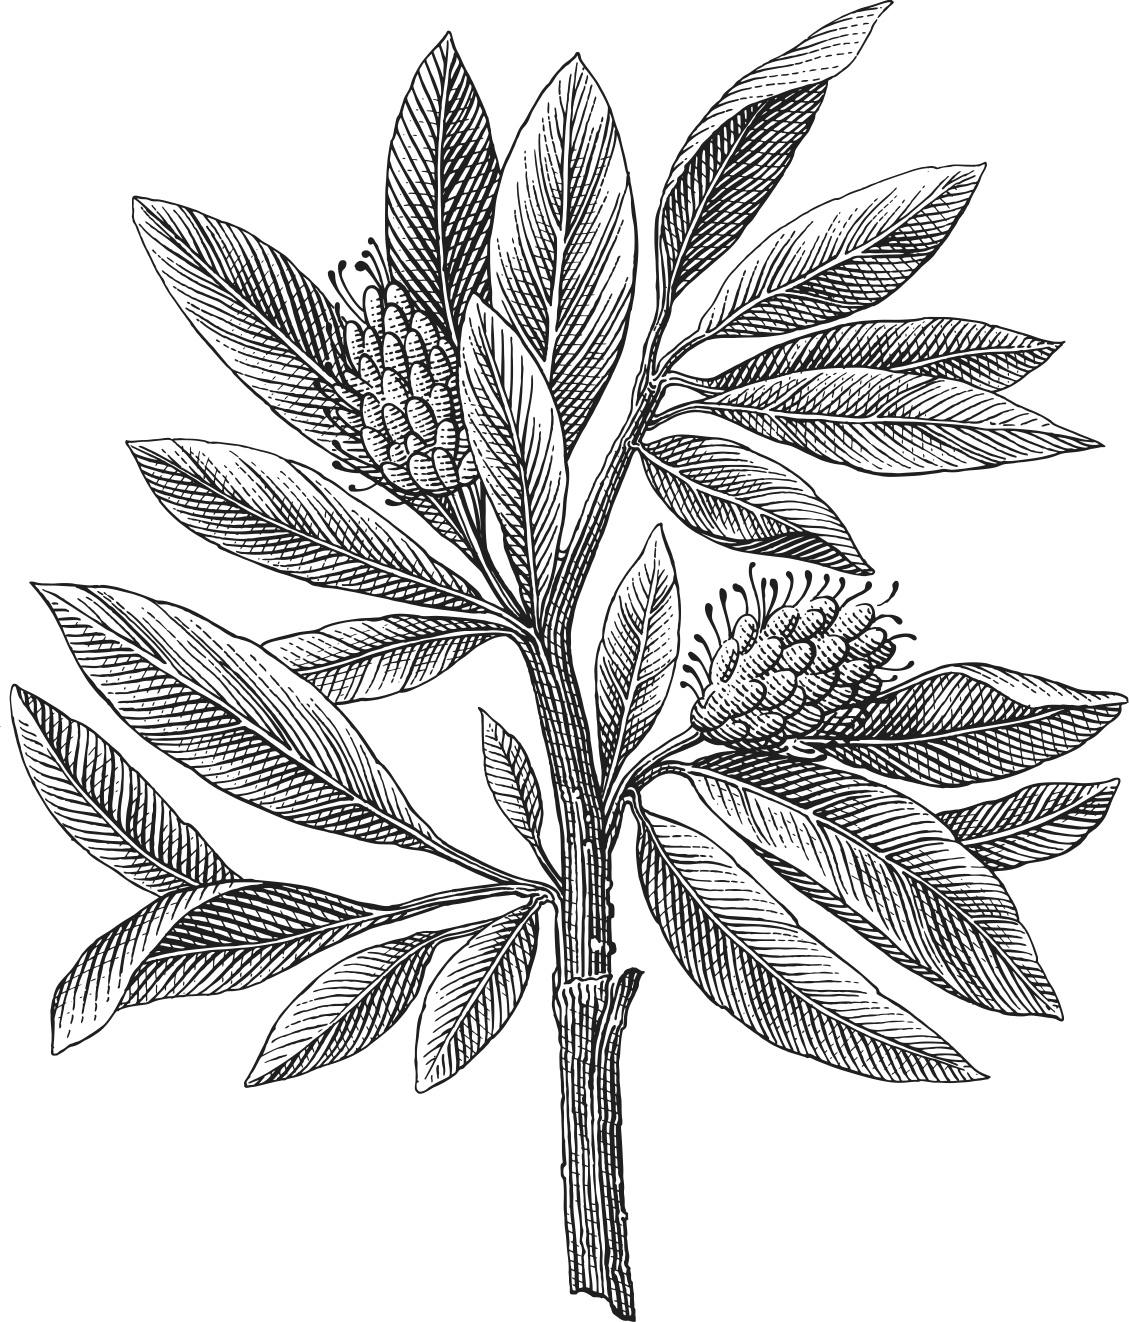
\includegraphics[keepaspectratio,scale=0.65]{lnu_etch.png} % Bakgrundsbild
    }
}
\newcommand\BackgroundPicLogo{
    \put(15,700){
    
\includegraphics[keepaspectratio,scale=0.10]{logo.png} % Logga i vänstra hörnet
    }	
}

\newcommand{\horrule}[1]{\rule{\linewidth}{#1}} % Skapa hortisontell linje

\title{	\vspace{-10cm}
    \normalfont \normalsize
    \textsc{Linnaeus University} \\ [25pt] % Universitetes namn
    \horrule{0.5pt} \\[0.4cm] % Tunn linje högst upp
    \huge Seminar 2\\ % Arbetes titel
	\large \textcolor{gray}{1DV720 -- Server Administration}
    \horrule{0.5pt} \\[0.4cm] % Tunn linje längst ner
}

\author{Jacob Lindehoff} % Författarnas namn

\date{\normalsize\today} % Dagens datum

\begin{document}
  \AddToShipoutPicture*{\BackgroundPic} % Lägger in backgrundsbild på första sidan
  \AddToShipoutPicture*{\BackgroundPicLogo}
  \maketitle % Skriv ut titeln
  \noindent % Tabba inte in på första meningen

  %------------------------------------------------
  % Introduktion
  %------------------------------------------------
  \section{Introduction}
  During this seminar, we will address the following topics:
  \begin{itemize}
    \item File Systems: NTFS, EXT
    \item Permissions, Local Users and Groups
    \item Storage – RAID
    \item File server - SMB and Samba
  \end{itemize}

  %------------------------------------------------
  %	Deadline
  %------------------------------------------------
  \section{Deadline}
  The seminar is on the {\color{red}8th of February 2016} and it is compulsory. If you cannot participate, it must be notified in advance and a written report of the seminar must be submitted no later than {\color{red}3 days} after the seminar. The written report should contain detailed answers to all questions in the seminar.
  \newpage

  %------------------------------------------------
  %	Seminariefrågor
  %------------------------------------------------
  \section{Seminar Questions}
  \subsection{File Systems}
  \begin{enumerate}
    \begin{large}
      \item Briefly describe:
      \begin{enumerate}[a.]
      	\item EXT
      	\item NTFS
      \end{enumerate}
      \item What additional functionality you get with NTFS when compared to FAT32?
      \item Can more than one user be the owner of a file or directory? Motivate your answer.
      	\begin{enumerate}[a.]
      		\item in Windows
      		\item in Linux
	    \end{enumerate}
      \item What are NTFS mounted drives?
      \item Does NTFS have support for symbolic links that are in e.g. Linux?
      \item What kind of filesystems does:
      \begin{enumerate}[a.]
      	\item Linux support to be run on?
      	\item Windows support to be run on? 
      \end{enumerate}
      \item Name two disadvantages with FAT32. Could it ever be a good idea to use FAT32 or ext2 in any context?
      \item What is a journaling filesystem?
      \setcounter{tmpc}{\theenumi}
    \end{large}
  \end{enumerate}

  \subsection{Permissions, Local Users and Groups}
  \begin{enumerate}
    \setcounter{enumi}{\thetmpc}
    \begin{large}
      \item What files are handling the users and groups in Linux? 
      \item Where are the passwords stored in Linux?
      \item What does the following linux commands do and how do you use them?
      \begin{enumerate}[a.]
      	\item chown
      	\item chgrp
      	\item chmod
      \end{enumerate}
	  \newpage      
      \item Using ls -l we get the following outcome from a directory:
		\begin{lstlisting}[style=BashInputStyle]
-rw-r--r--	1	adam		root	0	jan 26	20:36	file1
-rw-r--r--	1	bertil	root	0	jan 26	20:36	file2
drwxr-xr-x	1	ceasar	root	0	jan 26	20:36	folder1
		\end{lstlisting}
		\begin{enumerate}[a.]
      		\item What character denotes it is a folder?
      		\item (as superuser) What would be the permissions if you issued these commands:      chmod 750 file1. Explain what changes from the original permissions setting.
      		\item Including the changes from {b} would adam be able to access file1? If you also(as superuser) issued chown bertil file1.
      		\item If you want to recursively change the owner to Adam of all subfolders and files including fodler1 what command would you issue?
      		\item file2 contains supersecret company information that only bertil should be allowed to see and change. What permissions would you have to set that only Bertil can see it? Are there any other users that you can think of that this information cannot be hidden from?
      	\end{enumerate}
  	  \item Explain how permission inheritance works in NTFS?
      \item What is an ACL and what does it contain?
      \item What are cumulative NTFS permissions?
      \item What happens with the NTFS permissions when we:
      \begin{enumerate}[a.]
      	\item move a file within the same NTFS volume
      	\item copy a file within the same NTFS volume
      	\item move a file to another NTFS volume
      	\item copy a file to another NTFS volume
      \end{enumerate}

    \setcounter{tmpc}{\theenumi}
    \end{large}
  \end{enumerate}
  \newpage
  \subsection{Storage – RAID}
  \begin{enumerate}
    \setcounter{enumi}{\thetmpc}
    \begin{large}
      \item Explain what RAID is and list some different types of RAID solutions.
      \item Windows has different naming for RAID solutions, explain the following disk storage methods, how they work and when it is recommended to use them:
      \begin{enumerate}[a.]
        \item Simple
        \item Spanned
        \item Striped
        \item Mirrored
        \item RAID-5
      \end{enumerate}
    \setcounter{tmpc}{\theenumi}
    \end{large}
  \end{enumerate}

  \subsection{File server - SMB and Samba}
  \begin{enumerate}
    \setcounter{enumi}{\thetmpc}
    \begin{large}
      \item What are the differences between NTFS permissions and Share permissions?
      \begin{enumerate}[a.]
        \item Why do Share permissions exist when we can use the NTFS permissions instead?
      \end{enumerate}
	  \item Describe at least 3 ways to share a folder in Windows.
	  \item What are the big differences between the versions of SMB?
	  \item Describe the early days of samba and how it was developed.
	  \item What SMB(Server Message Block) versions does the current samba version support?
	  \item Describe 5 options in the smb.conf file and what they do.
	  \item The smb.conf manual describe 3 special sections: [global], [homes] and [printers] explain how they work.
	  \item What is swat in the samba suite?
    \setcounter{tmpc}{\theenumi}
    \end{large}
  \end{enumerate}

\end{document}
